%%%%%%%% ICML 2020 EXAMPLE LATEX SUBMISSION FILE %%%%%%%%%%%%%%%%%

\documentclass{article}

% Recommended, but optional, packages for figures and better typesetting:
\usepackage{microtype}
\usepackage{graphicx}
\usepackage{subcaption}
\usepackage{booktabs} % for professional tables
\usepackage{enumitem}
\setlist{nosep}
\usepackage{amsmath, amssymb, amsthm}

% hyperref makes hyperlinks in the resulting PDF.
% If your build breaks (sometimes temporarily if a hyperlink spans a page)
% please comment out the following usepackage line and replace
% \usepackage{icml2020} with \usepackage[nohyperref]{icml2020} above.
\usepackage{hyperref}

%multi-row
\usepackage{multirow}

% Attempt to make hyperref and algorithmic work together better:
\newcommand{\theHalgorithm}{\arabic{algorithm}}
\newcommand{\err}{\mathsf{err}}
\newcommand{\Aa}{\mathcal{A}}
\newcommand{\Dd}{\mathcal{D}}
\newcommand{\dd}{\mathbb{D}}
\newcommand{\Ff}{\mathcal{F}}
\newcommand{\Mm}{\mathcal{M}}

\theoremstyle{definition}
\newtheorem{definition}{Definition}[section]
\newtheorem{theorem}{Theorem}[section]
\newtheorem{corollary}{Corollary}[theorem]
\newtheorem{lemma}[theorem]{Lemma}

% Use the following line for the initial blind version submitted for review:
%\usepackage{icml2020}

% If accepted, instead use the following line for the camera-ready submission:
\usepackage[accepted]{icml2020}

% The \icmltitle you define below is probably too long as a header.
% Therefore, a short form for the running title is supplied here:
\icmltitlerunning{Foundation Model Features are Strong Baselines for Private Learning}

\begin{document}

\twocolumn[
\icmltitle{Foundation Model Features are Strong Baseline for Private Learning}

% It is OKAY to include author information, even for blind
% submissions: the style file will automatically remove it for you
% unless you've provided the [accepted] option to the icml2020
% package.

% List of affiliations: The first argument should be a (short)
% identifier you will use later to specify author affiliations
% Academic affiliations should list Department, University, City, Region, Country
% Industry affiliations should list Company, City, Region, Country

% You can specify symbols, otherwise they are numbered in order.
% Ideally, you should not use this facility. Affiliations will be numbered
% in order of appearance and this is the preferred way.
% \icmlsetsymbol{equal}{*}

\begin{icmlauthorlist}
\icmlauthor{Joon Suk Huh}{wics}
\icmlauthor{Yu Sun}{wimath}
\icmlauthor{Matthew Trefilek}{wics}
\end{icmlauthorlist}

\icmlaffiliation{wics}{Department of Computer Science, University of Wisconsin–Maidson, Madison, USA}
\icmlaffiliation{wimath}{Department of Mathmatics, University of Wisconsin–Maidson, Madison, USA}

\icmlcorrespondingauthor{Joon Suk Huh}{joon@cs.wisc.edu}

% You may provide any keywords that you
% find helpful for describing your paper; these are used to populate
% the "keywords" metadata in the PDF but will not be shown in the document
\icmlkeywords{Machine Learning, ICML}

\vskip 0.3in
]

% this must go after the closing bracket ] following \twocolumn[ ...

% This command actually creates the footnote in the first column
% listing the affiliations and the copyright notice.
% The command takes one argument, which is text to display at the start of the footnote.
% The \icmlEqualContribution command is standard text for equal contribution.
% Remove it (just {}) if you do not need this facility.

\printAffiliationsAndNotice{}  % leave blank if no need to mention equal contribution
%\printAffiliationsAndNotice{\icmlEqualContribution} % otherwise use the standard text.

\begin{abstract}
When it comes to machine learning, the alignment problem poses a complication for models trying to balance privacy and fairness. We propose three methods to achieve high accuracy while maintaining strong $\epsilon$-Differential Privacy bounds. By utilizing large pre-trained models, we extract features for new datasets and can train a diferentially private model over the extracted feature vectors. By doing this, we propose that we can obfuscate individual sample information and still maintain a high accuracy for low $\epsilon$ values when compared to previous benchmarks. In particular, our methods are able to produce state of the art results on the CIFAR-10, CIFAR-100, and Chest X-Ray datasets given a strong $\epsilon$ constraint.
\end{abstract}

\section{Introduction}
Aligning machine learning with human values such as privacy and fairness, known as the alignment problem \cite{christian2020alignment} is one of pre-eminent challenges in the field. While the alignment problem has only recently been defined, privacy and fairness in machine learning have been extensively studied topics in the last several years \cite{liu2021machine,mehrabi2021survey}. However, a common consensus is that aligning a model to social values often compromises the model's accuracy and efficiency. Moreover, a recent finding \cite{bagdasaryan2019differential} shows intrinsic tension between different values such as privacy and fairness; that is, aligning a model to one value (e.g. privacy) may harm the other value (e.g. fairness). Therefore, the practical research goals on the alignment problem are to understand the origin of such trade-offs and devise novel methods for better performance given social constraints.

In this paper, we look into a subproblem of the alignment problem, which is the problem of preserving privacy in machine learning systems. While there are several different approaches toward private machine learning, we mainly focus on differential privacy \cite{dwork2006differential}, which is a \textit{de facto} standard formalism of privacy in data science and machine learning. We formally introduce the notion of differentially private (DP) learning in Section \ref{subsec:dp}. An intuitive understanding of DP learning is as follows: the training algorithm should output similar models (or model parameters) for any given two training sets that only differ by one example. This requirement is parametrized by a parameter denoted as $\epsilon$ (see Definition \ref{def:dp})\footnote{$\delta$ is customarily set to $10^{-5}$.}, where it controls how two output distributions (over model parameters) are close to each other. Smaller $\epsilon$ indicates two distributions are indistinguishable. While there is no consensus on what value of $\epsilon$ should be considered as a safe guarantee of privacy, most works consider $\epsilon\in[1,10]$. In this work, we consider $\epsilon<1.0$ as the strong privacy regime.

In Section \ref{subsec:related}, we build up our main thesis by introducing relevant works. In Section \ref{subsec:maincont}, we summarize our contributions. In Section \ref{sec:prelim}, we introduce a set of notations and the formal notion of differentially private learning. In Section \ref{subsec:featext}, we introduce feature extractors used in our experiment. In Section \ref{subsec:theory}, we informally state our theoretical contribution. In Section \ref{subsec:exp}, we benchmark our new baseline methods and show that they outperform existing methods by large margins in natural datasets such as CIFAR-10 and CIFAR-100.

\subsection{Related Works}
\label{subsec:related}
The seminal work of \cite{abadi2016deep} first demonstrated practical private training of deep learning models by inventing a tool called ``moment accountant". Moment accountant is a set of convenient mathematical rules that allows one to track DP parameters along each training step. The moment accountant technique is implemented in standard DP deep learning frameworks such as Opacus \cite{yousefpour2021opacus} and TF Privacy \cite{abadi2016tensorflow}.

Even after the initial breakthrough by \cite{abadi2016deep} and recent breakthrough by \cite{luo2021scalable}, DP deep learning methods are still remained to be unscalable to real-world datasets due to their slow convergence and low accuracy. So why do deep learning and DP not work together on real-world datasets? Recent theoretical \cite{feldman2020does, brown2021memorization} and experimental works \cite{feldman2020neural} suggest that real-world datasets are mixtures of subpopulations whose occurrence statistics are long-tailed. Long-tailness of real-world datasets implies that any accurate learner should memorize examples from each subpopulation. From this point of view, DP learners cannot achieve good accuracies as DP constraints prevent them from memorizing training examples. 

The most relevant work to ours is \cite{tramer2020differentially}. This work argues that modern DP deep learning methods have not yet achieved the 'AlexNet' moment by showing that a linear classifier over features extracted from a simple handcrafted feature extractor \cite{oyallon2015deep} can easily outperform deep neural network-based classifiers in DP setting.

\subsection{Main Contributions}
\label{subsec:maincont}
We develop our main point from \cite{tramer2020differentially}. We argue that large-scale pre-trained networks such as Vision Transformer (ViT) \cite{dosovitskiy2020image} and CLIP \cite{radford2021learning} are exceptionally good feature extractors for private learning. Specifically,
\begin{enumerate}
    \item We show that a linear classifier trained with features extracted from ViT and CLIP can outperform state-of-the-arts in realistic datasets such as CIFAR-10 and CIFAR-100.
    \item We prove that under a certain long-tail condition on data distribution, it is impossible to achieve both high accuracy and privacy (Informally stated in Theorem \ref{thm:main}).
\end{enumerate}

Our method can be seen as a simplification of the DP learning strategy of utilizing public datasets. Public datasets can help private learning by allowing classifiers to learn features (inductive bias) within the target domain with less access to the private dataset. This strategy has been adopted in state-of-the-art methods like PATE \cite{papernot2018scalable} and Sparse Network Finetuning \cite{luo2021scalable}. 

We denote features from large-scale pre-trained models as ``foundation model'' features following the term coined in \cite{bommasani2021opportunities}. Foundation models (e.g. GPT-3, BERT, ViT and CLIP) are large-scale deep neural networks trained over large-scale datasets. A common feature among foundation models is that they generalize to unseen tasks from few examples. This capability of foundation models suggest that they can help building better private models as suggested in \cite{bommasani2021opportunities}.

Finally, our theoretical result (Theorem \ref{thm:main}) suggests that foundation model features are not long-tailed as there is a fundamental tension between accuracy and privacy in long-tailed distribution. This result can guide us to build better feature extractors for differentially private learning by regulating the long-tailness of extracted features.

\section{Preliminary}
\label{sec:prelim}

\subsection{Notations}
\label{sec:not}
Let $D=\left\{(x_i,y_i\right\}_{i=1}^N$ be labeled dataset of size $N$. We denote $\Dd$ as the set of all possible labeled datasets and $\Ff$ as the set of machine learning models. Also we denote $\Delta(\Ff)$ as the set of all probability distributions over $\Ff$. With these notations, we formalize any randomized training algorithm $\Mm$ as a map $\Mm:\Dd\rightarrow\Delta(\Ff)$. As most training algorithms (e.g. SGD) are not deterministic, this gives the most general formalism.

\subsection{Differentially Private Learning}
\label{subsec:dp}
\begin{definition}[Differentially Private Learning] We say the learning algorithm $\Mm:\Dd\rightarrow\Delta(\Ff)$ satisfies $(\epsilon, \delta)$-differential privacy, if for any training sets $D$, $D'$ that differ in one example, and any $S\subseteq\Ff$: 
\begin{align}
    \Pr\left[\Mm(D)\in S \right]\leq e^\epsilon \Pr\left[\Mm(D')\in S\right]+\delta,
\end{align}
where $\epsilon$ controls how two distributions $\Mm(D)$ and $\Mm(D')$ are close to each other and $\delta$ controls the chance of the mechanism $\Mm$ fails to be private.
\label{def:dp}
\end{definition}
It is customary to set $\delta=10^{-5}$. We follow this custom and use Opacus framework\cite{yousefpour2021opacus} to track $\epsilon$ parameter given $\delta=10^{-5}$.

\subsection{Feature Extractors}
\label{subsec:featext}
In this section, we breifly introduce our main method. As mentioned in Section \ref{subsec:maincont}, our method is a linear classifier over features extracted from ResNet50, ViT and CLIP. Due to it's simplicity, we propose our method as a new baseline. Dimensions of extracted features are listed in Table \ref{tab:embedded_dims}. We use Opacus framework to train linear classifiers. Since naive hyper-parameter optimizations suffer from privacy leaks, one has to adopt differentially private version of hyper-parameter optimization \cite{liu2019private, priyanshu2021efficient}. We circumvent this problem by fixing the hyper-parameters before seeing the test performance. We choose $\textsf{Batch\_Size}=32$, $\textsf{Number\_of\_Epochs}=20$, $\textsf{Learning\_Rate}=0.1$ and $\textsf{Maximum\_Gradient\_Norm}=1.2$.

\section{Results}
\subsection{Theoretical Results}
\label{subsec:theory}
In this section, we informally state the main theorem that gives a negative result on training a private classifier over long-tailed distribution.
\begin{theorem}[Informal]
    Let $M$ be the number of subclasses in long-tailed data distribution. Any sufficiently well-behaving training algorithms are $\epsilon$-differentially private with $\epsilon \geq M\ln N$, where $N$  is the size of training set.
    \label{thm:main}
\end{theorem}
The full version of Theorem \ref{thm:main} and its proof can be found in the supplementary material (Theorem 2.1).

\subsection{Experiment Results}
\label{subsec:exp}

We designed our experiment based on the experiment described in \citet{tramer2020differentially}. We have selected a number of datasets and have chosen pre-trained models that we will extract the final layer from. The models chosen are ResNet50 \cite{he2016deep}, ViT \cite{dosovitskiy2020image}, and CLIP \cite{radford2021learning}. The penultimate layer was chosen, and for each batch of images sent through the models, we extracted a feature vector the size represented in Table \ref{tab:embedded_dims}. This feature vector represents the embedding of a given image before any activation functions are employed. For CLIP, a vector of sentences was generated using the following form: "This is a picture of a/an CLASS". For MNIST we replaced the classtext with: "This is the number CLASS". For EuroSAT and Chest X-Ray we explicit told clip it was a satellite image or x-ray respectively.

\begin{table}[h]
    \centering
    \begin{tabular}{c|c}
        Pre-Trained Model & Output Dimension \\
        \toprule
        ResNet50 &  2048 \\
        ViT & 768 \\
        CLIP & 512\\
    \end{tabular}
    \caption{Dimensions of the extracted layers.}
    \label{tab:embedded_dims}
\end{table}


For our chosen datasets, we then trained a differentially private linear classifier using the extracted features as our input. Our hyperameters were a chosen $\epsilon$, $\delta$ of $10^{-5}$, 20 epochs, and a learning rate of $0.1$. The Datasets chosen were MNIST, Fashion-MNIST, and CIFAR-10 for comparison against \cite{tramer2020differentially}. PlantDisease and EuroSAT for comparison against \cite{luo2021scalable}. Chest X-Ray for comparison against \cite{ziller2021medical}. We chose CIFAR-100 as another dataset for which there is not a baseline comparison. The test results are compared to the baseline measurements as well as their respective $\epsilon$-Differential Privacy scores. The linear classifier was programmed using pyTorch and Opacus for the utilities provided to measure the moment accountant. Then, the linear classifiers were trained and tested using a split made up of extracted features.

\subsection{Analysis}
\begin{table*}[ht!]
	\centering
	\footnotesize
	\begin{tabular}{@{} l l l r r r r r r@{}}
		& & & \multicolumn{5}{c}{Performance (Accuracy $\%$ or AUC)}\\
		\cmidrule{4-9}
		Data & $\epsilon$-DP & Source & CNN & SN+LC & SN+CNN & ResNet50+LC & ViT+LC & CLIP+LC \\
		\toprule
				
		\multirow{7}{5em}{MNIST}
		&1.2 & \citet{feldman2020individual} & $96.6$ & $\bf{98.1}$ & $97.8$ & $91.8$ & $94.9$ & $95.5$ \\
		&2.0 & \citet{abadi2016deep} & $95.0$ & $\bf{98.5}$ & $98.4$\\
		&2.32 & \citet{bu2020deep} & $96.6$ & $\bf{98.6}$ & $98.5$\\
		&2.5 & \citet{chen2020stochastic} & $90.0$ & $\bf{98.7}$ & $98.6$\\
		&2.93 & \citet{papernot2020making} &$98.1$ & $\bf{98.7}$ & $\bf{98.7}$\\
		&3.2 & \citet{nasr2020improving} & $96.1$ & -- \\ % 98.7
		&6.78 & \citet{yu2019differentially} & $93.2$ & --\\% 98.9-99.0
		\midrule

		\multirow{2}{5em}{Fashion-MNIST}
		&2.7 & \citet{papernot2020making} &$86.1$ & $\bf{89.5}$ & $88.7$ & $83.6$ & $88.1$ & $86.0$\\
		&3.0 & \citet{chen2020stochastic} & $82.3$ & $\bf{89.7}$ & $89.0$ \\
		\midrule
		
		\multirow{4}{5em}{CIFAR-10}
		&0.5 & \citet{luo2021scalable} & $73.3$ & -- & -- & 49.7 & \bf{94.0} & 92.7 \\
		&3.0 & \citet{nasr2020improving} & $55.0$ & ${67.0}$ & $69.3$\\
		&6.78 & \citet{yu2019differentially} & $44.3$ & -- &--\\ % ~68
		&7.53 & \citet{papernot2020making} &$66.2$ & -- & --\\ % ~69
		&8.0 & \citet{chen2020stochastic} & $53.0$ & -- & --\\
		\midrule
		
		\multirow{1}{5em}{CIFAR-100}
		&0.5 & This work & -- & -- & -- & 16.2 & \bf{72.0} & 60.05 \\
        \midrule
		
		\multirow{1}{5em}{PlantDisease}
		&0.5 & This work & -- & -- & -- & 83.7 & \bf{92.1} & 87.1 \\
		&$[0.5, 1.5]$ & \citet{luo2021scalable} & \bf{97.9} & -- & -- & & &  \\
        \midrule
        
		\multirow{1}{5em}{EuroSAT}
		&0.5 & This work & -- & -- & -- & 78.9 & \bf{89.9} & 88.8 \\
		&$[0.5, 1.5]$ & \citet{luo2021scalable} & \bf{90.1} & -- & -- & & &  \\
		\midrule	
		
		\multirow{1}{5em}{Chest X-Ray (AUC)}
		&0.5 & This work & -- & -- & -- & 0.92 & \bf{0.94} & 0.74 \\
		&0.52 & \citet{ziller2021medical} & $0.85$ \\
		&2.69 & \citet{ziller2021medical} & $0.88$ \\
		\bottomrule
	\end{tabular}
	\caption{A comparison of proposed differentially private methods in comparison to previous diferentially private CNN implementations. SN represents the results of ScatterNet proposed in \citet{tramer2020differentially}. LC and CNN abbreviations represent Linear Classifiers and Convolutional Neural Networks respectively that have been trained on top of the extracted features. ResNet50+LC, ViT+LC, and CLIP+LC represent our contributed methods.}
	\label{tab:results}
\end{table*}

The results from the Linear Classifiers are shown in Table \ref{tab:results}. We see that for MNIST and Fashion MNIST, ScatterNet performs better at the lowest $\epsilon$ values. For CIFAR-10, our ViT and CLIP extracted models perform better than both previous attempts with CNNs and ScatterNet for both accuracy and $\epsilon$-DP values. For CIFAR-100 we were able to maintain above a $70\%$ accuracy while maintaining an $\epsilon$ of $0.5$. Compared to \cite{luo2021scalable} our accuracy was lower, but our static $\epsilon$ of 0.5 guarantees stronger privacy than the range provided for the PlantDisease and EuroSAT accuracies. Our ViT-LC classifier was able to come within $0.2\%$ of their work for EuroSAT. Our ViT-LC and ResNet50-LC had lower Area Under the ROC Curve (AUC) scores for the Chest X-Ray Dataset than the CNN proposed by \cite{ziller2021medical} while maintaining a lower $\epsilon$-DP. For all tests performed on the Chest X-Ray, we measure performance in AUC to match the reports found in \cite{ziller2021medical}. The Chest X-Ray results are particularly promising because it is the smallest dataset we tested (5,232 images). It also was the only medical dataset, so the real world application of the alignment principle is very relevant. We want to protect the patient's information, but also want to deliver the best possible result for an individual.

From the benchmark results displayed in Table \ref{tab:results}, we can see the privacy tradeoff for accuracy: as the bound of $\epsilon$ weakens ($\epsilon$ increases) accuracy increases for ScatterNet. We show in Figure \ref{fig:acc_epsilon} that the tradeoff exists with our models as well. By loosening the restriction on $\epsilon$ for our methods on the CIFAR-10 dataset, we see accuracy increase for all three. ResNet50 has the largest growth, whereas ViT and CLIP both maintain a small margin in their accuracy.

Using t-SNE we were able to perform a visual analysis on how well the extracted features clustered when reduced to two dimensions. Figure \ref{fig:tsne} gives the plots for CIFAR-10 and Chest X-Ray for our three different feature extracting methods. It is clear that the visual distribution of the feature vectors matches the accuracy differences of our trained linear classifier. As we move from Resnet50 to CLIP to ViT, the clusters become more pronounced, specifically for CIFAR-10 where we saw performance better than previous benchmarks.

A final benchmark we conducted was producing a chart of non-DP bound accuracy scores for an N-Shot classifier built on top of CLIP. This method is not guaranteed to fall under any $(\epsilon,\delta)$-DP comparisons. By comparing the best accuracy scores from the experiment (all datasets performed best at the Full-Shot benchmark) to our Differentially Private accuracy scores, we can get an understanding of how much the tradeoff demonstrated in Figure \ref{fig:acc_epsilon} is affecting our accuracy results. Surprisingly, we can see that we are actually pushing the bounds for $\epsilon$ bound methods. Table \ref{tab:results_nondp} gives us scores for many of the datasets that are very close to our $\epsilon$-DP bound accuracies. Chest X-Ray, our state of the art differentially private method actually performed better than the non-DP N-Shot classifiers. CIFAR-10 and CIFAR-100 which were also achieved  high accuracy compared to the benchmarks fell within a few percentage points of the non-DP classifier.

\begin{figure}[h]
    \centering
    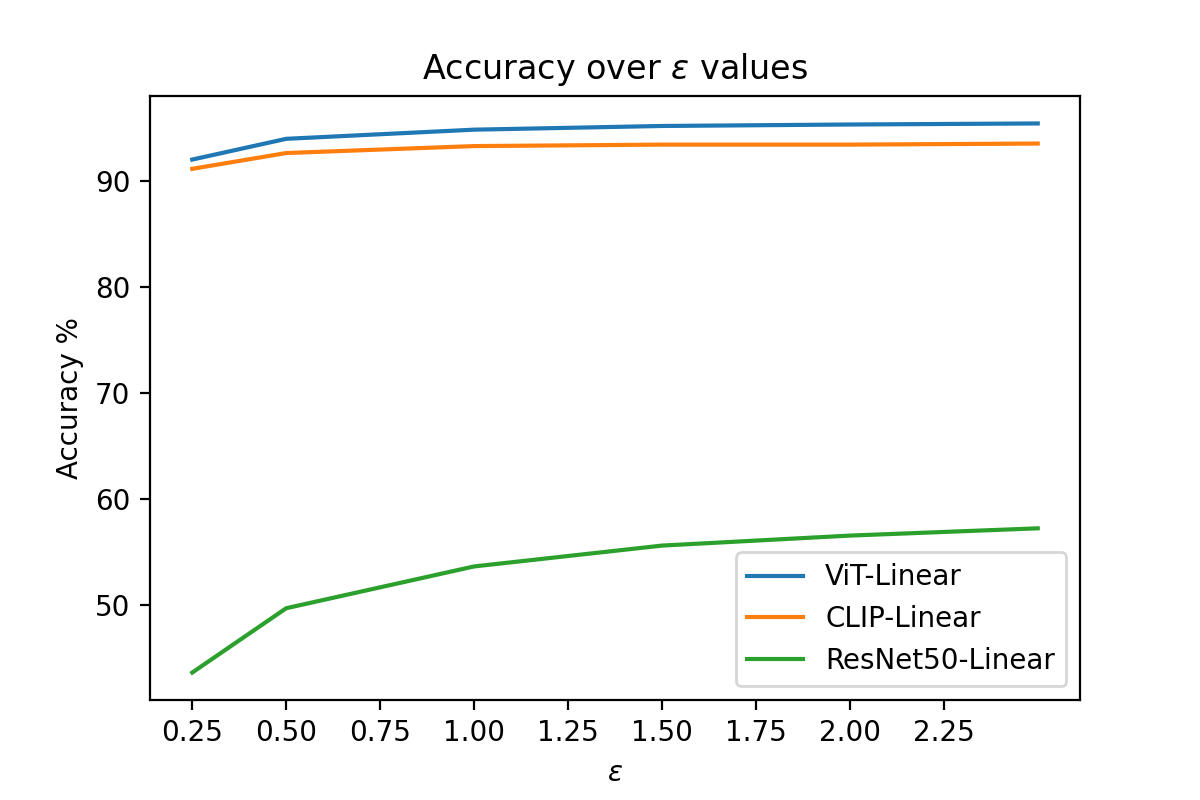
\includegraphics[width=.4\textwidth]{Final project/img/acc_epsilon.png}
    \caption{$\epsilon$'s effect on accuracy for the CIFAR-10 Dataset.}
    \label{fig:acc_epsilon}
\end{figure}

\begin{table*}[h!]
	\centering
	\footnotesize
	
	\begin{tabular}{@{} l r r r r r r @{}}
		& \multicolumn{6}{c}{Performance (Accuracy $\%$ or AUC)}\\
		\cmidrule{2-7}
		Data & Full & 0-Shot & 5-Shot & 10-Shot & 30-Shot & 100-Shot \\
		\toprule
		
		MNIST & 98.64 & 11.70 & 78.86 & 88.50 & 94.17 & 95.92 \\
		Fashion-MNIST & 90.22 & 60.32 & 69.96 & 77.63 & 82.40 & 85.91 \\
		CIFAR-10 & 94.67 & 88.41 & 84.25 & 89.44 & 91.22 & 92.69 \\
		CIFAR-100 & 78.94 & 60.25 & 55.70 & 62.99 & 70.34 & 75.44 \\
		PlantDisease & 98.32 & 10.60 & 75.50 & 82.54 & 90.31 & 94.52 \\
		EuroSAT & 95.44 & 28.89 & 74.96 & 80.33 & 88.48 & 91.74 \\
		ChestXRay (AUC) & 0.97 & 0.51 & 0.72 & 0.86 & 0.90 & 0.93 \\
		
		\bottomrule
	\end{tabular}
	
	\caption{A comparison of the accuracies of our $K$-Shot Classifier.}
	\label{tab:results_nondp}
\end{table*}

\begin{figure*}[h!]
    \centering
    \begin{subfigure}{.48\textwidth}
        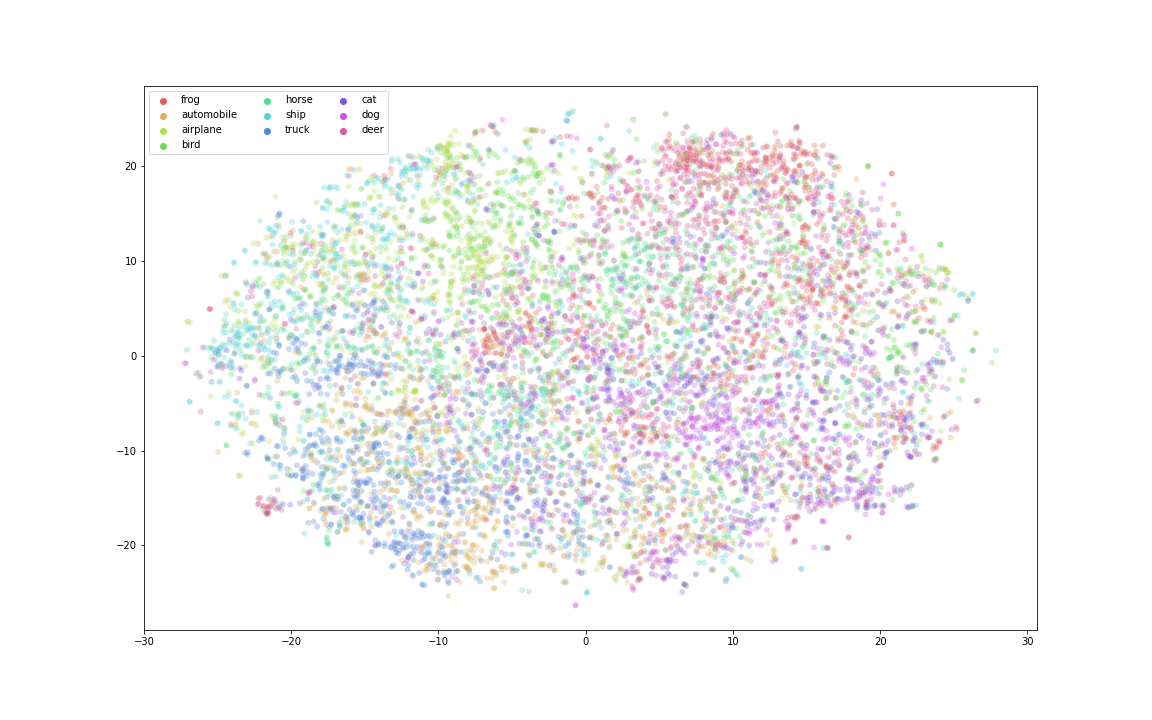
\includegraphics[width=\linewidth]{Final project/img/CIFAR10_RESNET50_train.png}
        \caption{ResNet50 - CIFAR-10}
    \end{subfigure}
    \begin{subfigure}{.48\textwidth}
        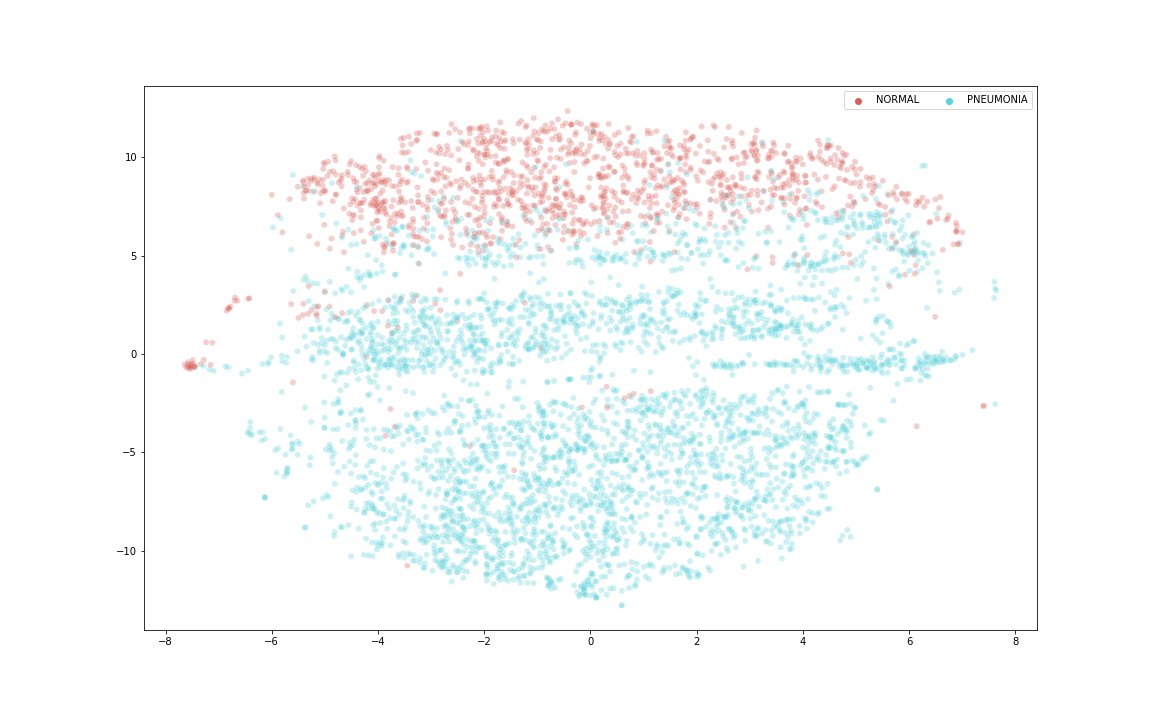
\includegraphics[width=\linewidth]{Final project/img/ChestXRay_RESNET50_train.png}
        \caption{ResNet50 - Chest X-Ray}
    \end{subfigure}
    \begin{subfigure}{.48\textwidth}
        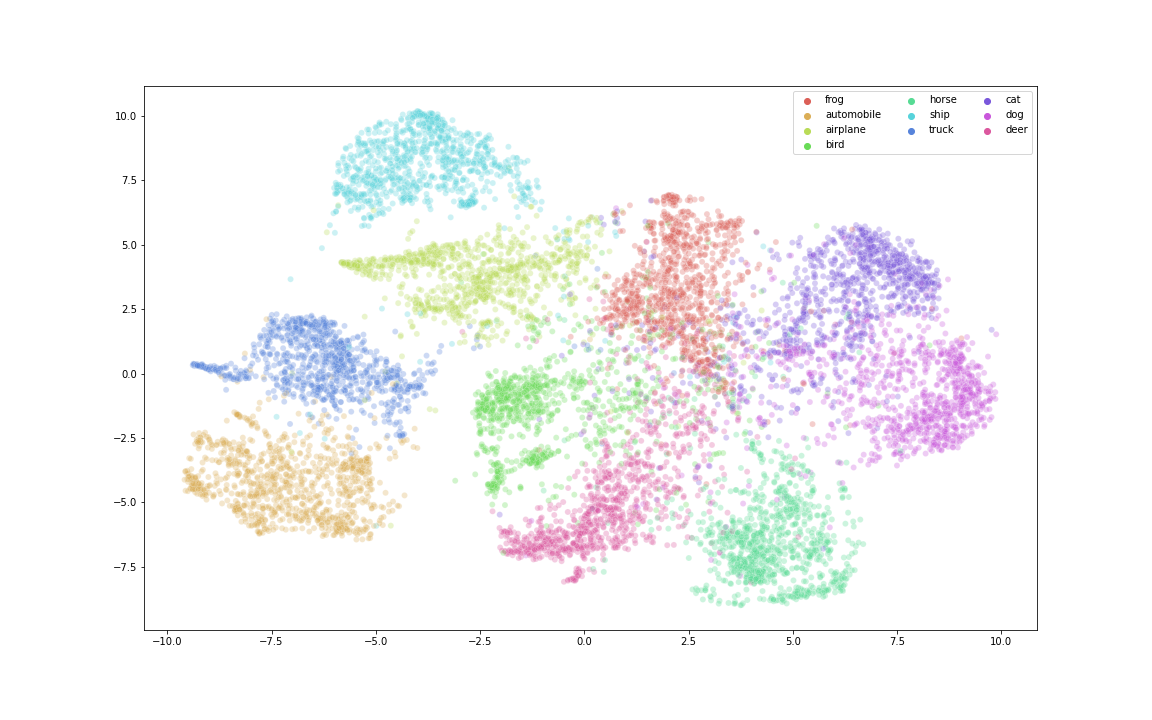
\includegraphics[width=\linewidth]{Final project/img/CIFAR10_clip-vit-base-patch32_train.png}
        \caption{CLIP - CIFAR-10}
    \end{subfigure}
    \begin{subfigure}{.48\textwidth}
        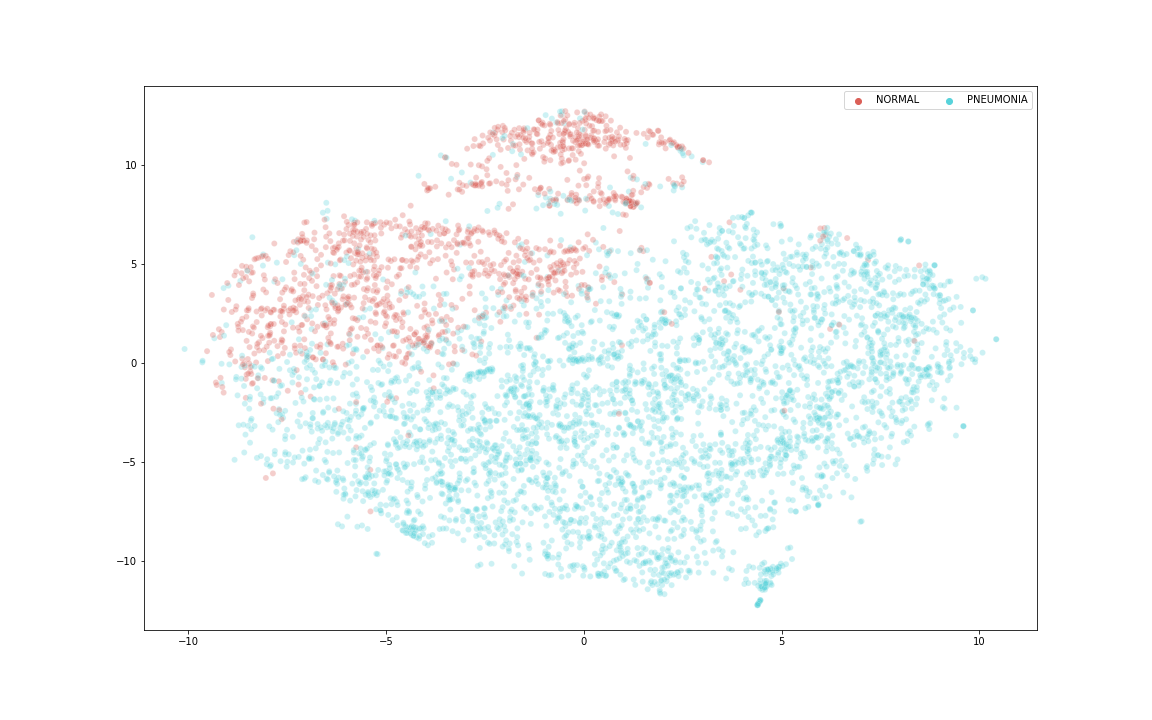
\includegraphics[width=\linewidth]{Final project/img/ChestXRay_clip-vit-base-patch32_train.png}
        \caption{CLIP - Chest X-Ray}
    \end{subfigure}
    \begin{subfigure}{.48\textwidth}
        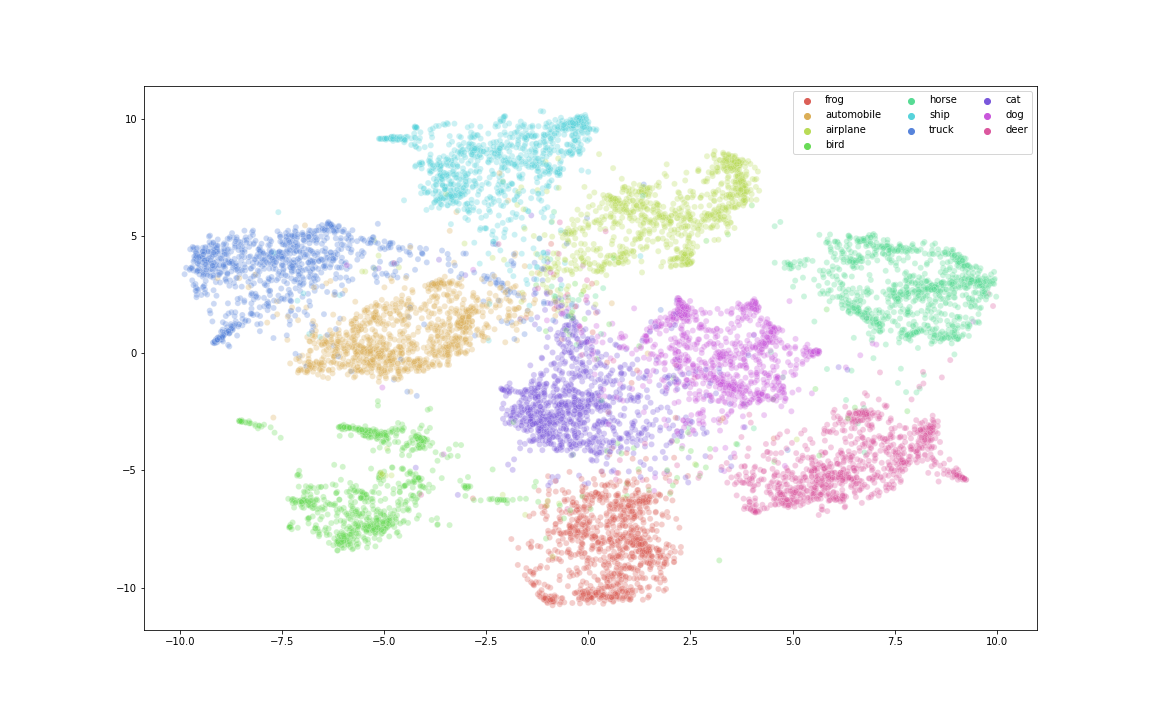
\includegraphics[width=\linewidth]{Final project/img/CIFAR10_vit-base-patch32-384_train.png}
        \caption{ViT - CIFAR-10}
    \end{subfigure}
    \begin{subfigure}{.48\textwidth}
        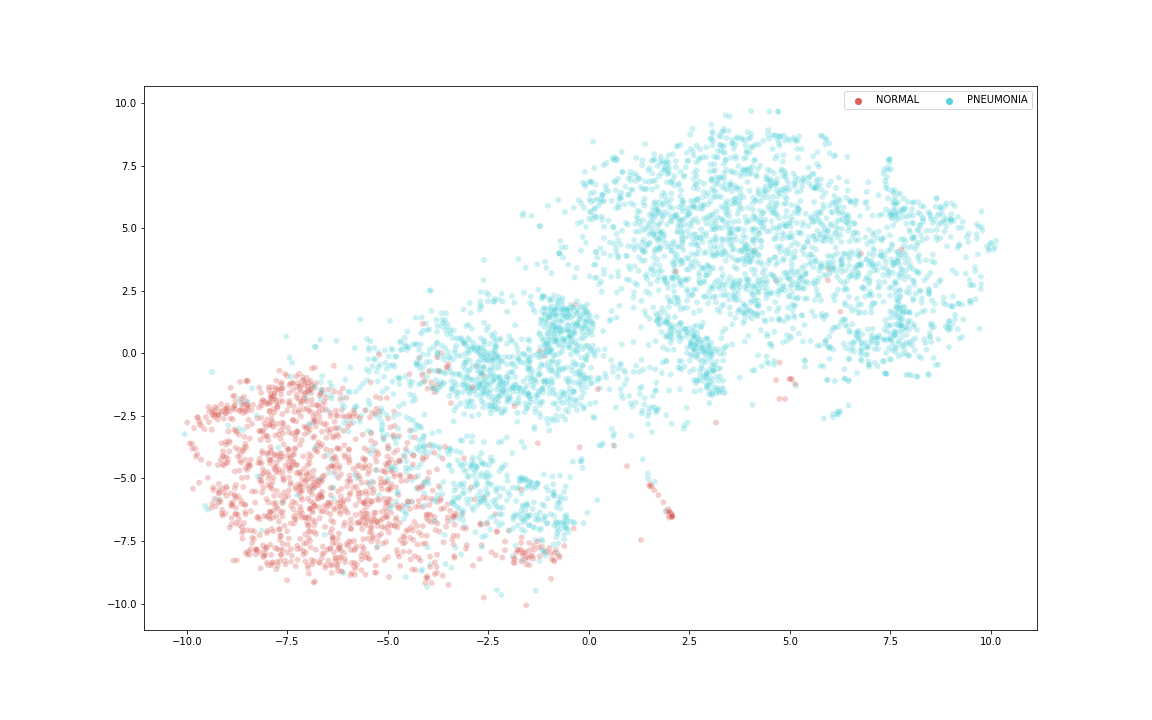
\includegraphics[width=\linewidth]{Final project/img/ChestXRay_vit-base-patch32-384_train.png}
        \caption{ViT - Chest X-Ray}
    \end{subfigure}
    \caption{t-SNE Plots for CIFAR-10 and Chest X-Ray}
    \label{fig:tsne}
\end{figure*}

\section{Conclusion}

In conclusion, we show that large-scale pre-trained networks are good feature extractors for private learning. We show that for CIFAR-10 and CIFAR-100, we can achieve new accuracy benchmarks at very low $\epsilon$-DP values. We also show that for small datasets where Differential Privacy becomes very important, e.g. Chest X-Ray, the abstraction into feature vectors can protect an individual's privacy by introducing a better AUC for a lower $\epsilon$ than previous studies.

We also posit that for certain long-tail conditions on data distributions that make it impossible to optimize both accuracy and privacy. Because of this, methods that value privacy and can achieve reasonable accuracy present the best case scenario in approaching the alignment problem.

\section{Contribution}
$40\%$: Joon; $30\%$: Matt; $30\%$: Yu;


Joon and Matt conducted the experiments and wrote the main body of the paper. Yu proved Theorem \ref{thm:main} and wrote the supplementary material.

% Note use of \abovespace and \belowspace to get reasonable spacing
% above and below tabular lines.

% \begin{algorithm}[tb]
%   \caption{Bubble Sort}
%   \label{alg:example}
% \begin{algorithmic}
%   \STATE {\bfseries Input:} data $x_i$, size $m$
%   \REPEAT
%   \STATE Initialize $noChange = true$.
%   \FOR{$i=1$ {\bfseries to} $m-1$}
%   \IF{$x_i > x_{i+1}$}
%   \STATE Swap $x_i$ and $x_{i+1}$
%   \STATE $noChange = false$
%   \ENDIF
%   \ENDFOR
%   \UNTIL{$noChange$ is $true$}
% \end{algorithmic}
% \end{algorithm}

% \begin{table}[t]
% \caption{Classification accuracies for naive Bayes and flexible
% Bayes on various data sets.}
% \label{sample-table}
% \vskip 0.15in
% \begin{center}
% \begin{small}
% \begin{sc}
% \begin{tabular}{lcccr}
% \toprule
% Data set & Naive & Flexible & Better? \\
% \midrule
% Breast    & 95.9$\pm$ 0.2& 96.7$\pm$ 0.2& $\surd$ \\
% Cleveland & 83.3$\pm$ 0.6& 80.0$\pm$ 0.6& $\times$\\
% Glass2    & 61.9$\pm$ 1.4& 83.8$\pm$ 0.7& $\surd$ \\
% Credit    & 74.8$\pm$ 0.5& 78.3$\pm$ 0.6&         \\
% Horse     & 73.3$\pm$ 0.9& 69.7$\pm$ 1.0& $\times$\\
% Meta      & 67.1$\pm$ 0.6& 76.5$\pm$ 0.5& $\surd$ \\
% Pima      & 75.1$\pm$ 0.6& 73.9$\pm$ 0.5&         \\
% Vehicle   & 44.9$\pm$ 0.6& 61.5$\pm$ 0.4& $\surd$ \\
% \bottomrule
% \end{tabular}
% \end{sc}
% \end{small}
% \end{center}
% \vskip -0.1in
% \end{table}

% Acknowledgements should only appear in the accepted version.
% \section*{Acknowledgements}


% In the unusual situation where you want a paper to appear in the
% references without citing it in the main text, use \nocite
\nocite{langley00}

\bibliography{ref}
\bibliographystyle{icml2020}


%%%%%%%%%%%%%%%%%%%%%%%%%%%%%%%%%%%%%%%%%%%%%%%%%%%%%%%%%%%%%%%%%%%%%%%%%%%%%%%
%%%%%%%%%%%%%%%%%%%%%%%%%%%%%%%%%%%%%%%%%%%%%%%%%%%%%%%%%%%%%%%%%%%%%%%%%%%%%%%
% DELETE THIS PART. DO NOT PLACE CONTENT AFTER THE REFERENCES!
%%%%%%%%%%%%%%%%%%%%%%%%%%%%%%%%%%%%%%%%%%%%%%%%%%%%%%%%%%%%%%%%%%%%%%%%%%%%%%%
%%%%%%%%%%%%%%%%%%%%%%%%%%%%%%%%%%%%%%%%%%%%%%%%%%%%%%%%%%%%%%%%%%%%%%%%%%%%%%%
\appendix
\begin{figure*}[h!]
    \centering
    \begin{subfigure}{.48\textwidth}
        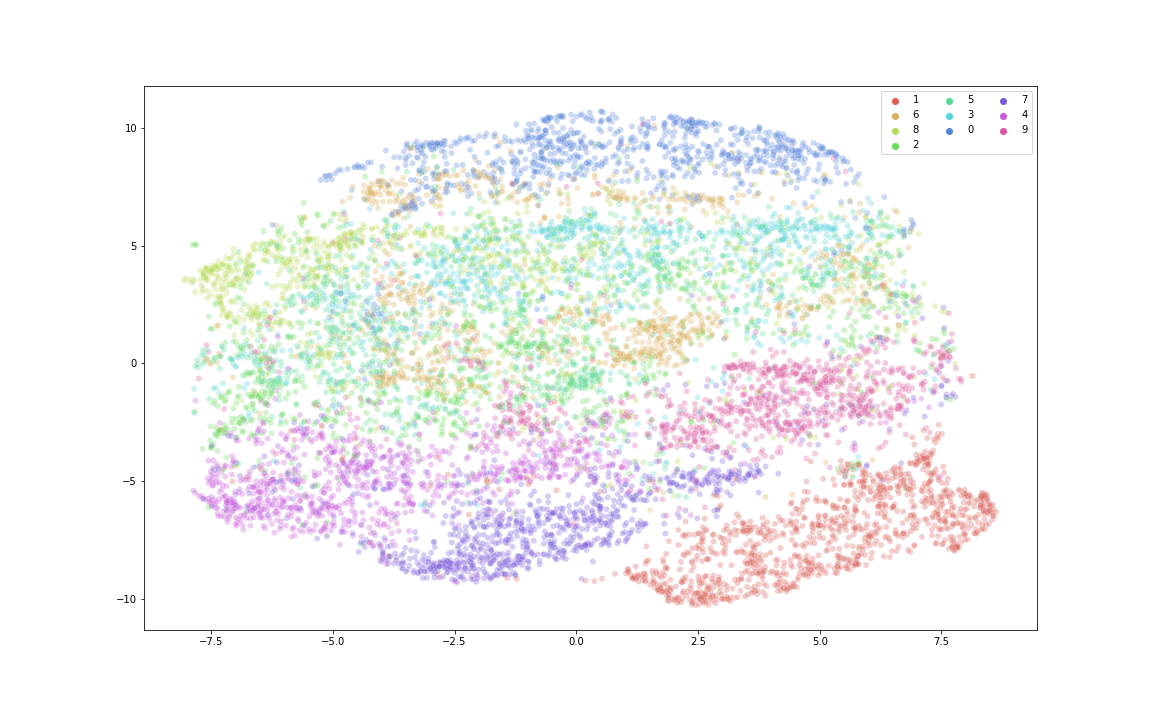
\includegraphics[width=\linewidth]{Final project/img/MNIST_RESNET50_train.png}
        \caption{ResNet50 - MNIST}
    \end{subfigure}
    \begin{subfigure}{.48\textwidth}
        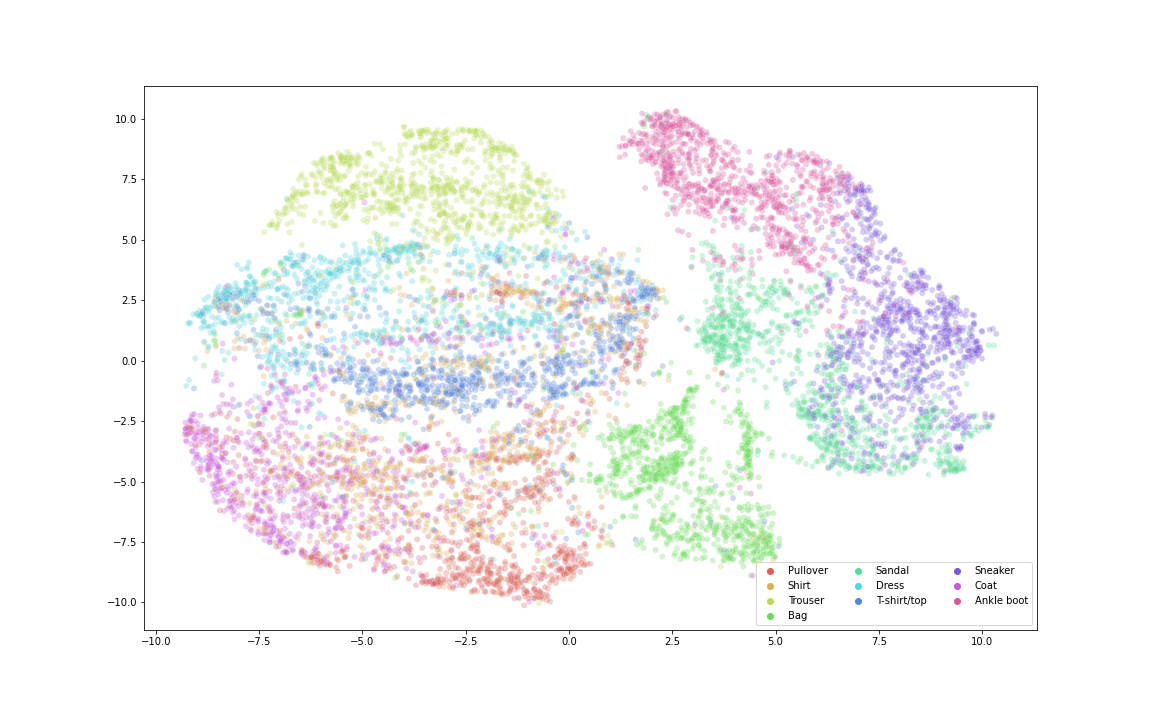
\includegraphics[width=\linewidth]{Final project/img/FMNIST_RESNET50_train.png}
        \caption{ResNet50 - FMNIST}
    \end{subfigure}
    \begin{subfigure}{.48\textwidth}
        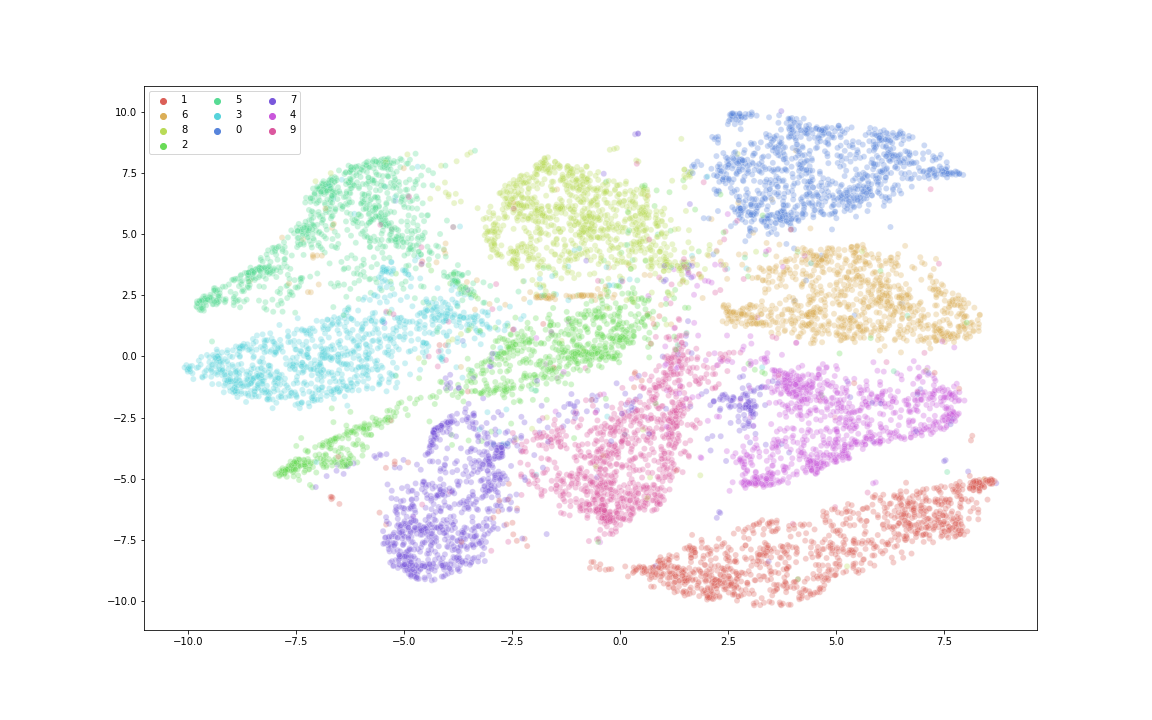
\includegraphics[width=\linewidth]{Final project/img/MNIST_clip-vit-base-patch32_train.png}
        \caption{CLIP - MNIST}
    \end{subfigure}
    \begin{subfigure}{.48\textwidth}
        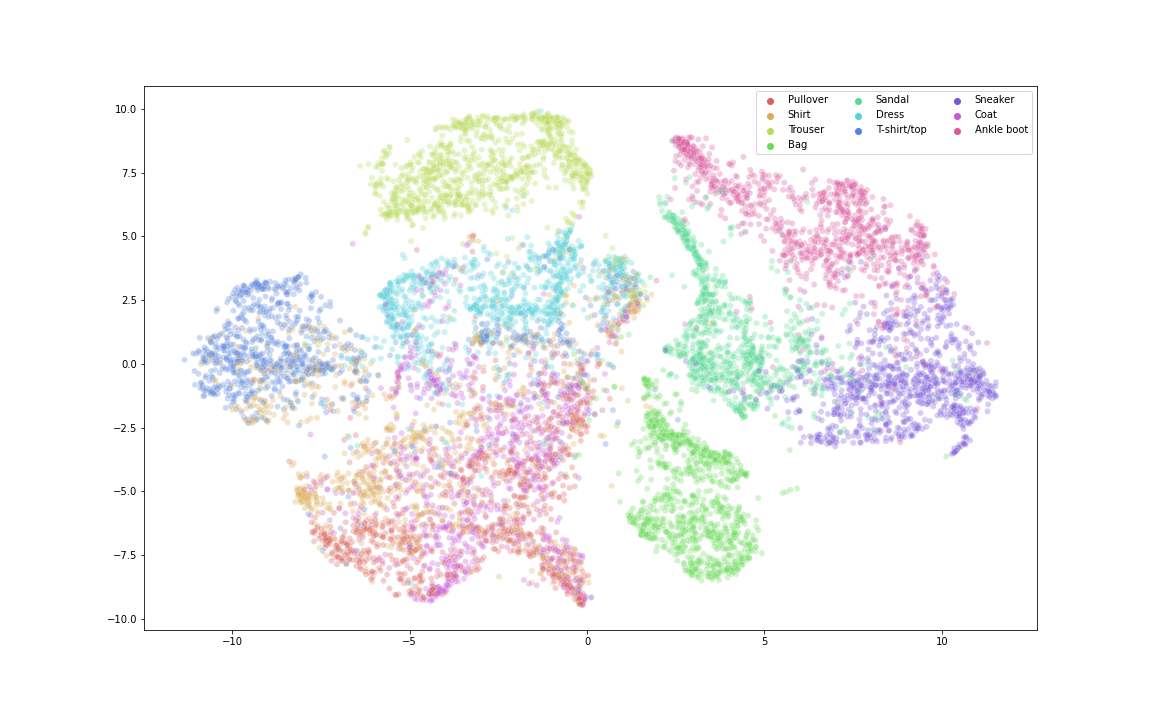
\includegraphics[width=\linewidth]{Final project/img/FMNIST_clip-vit-base-patch32_train.png}
        \caption{CLIP - FMNIST}
    \end{subfigure}
    \begin{subfigure}{.48\textwidth}
        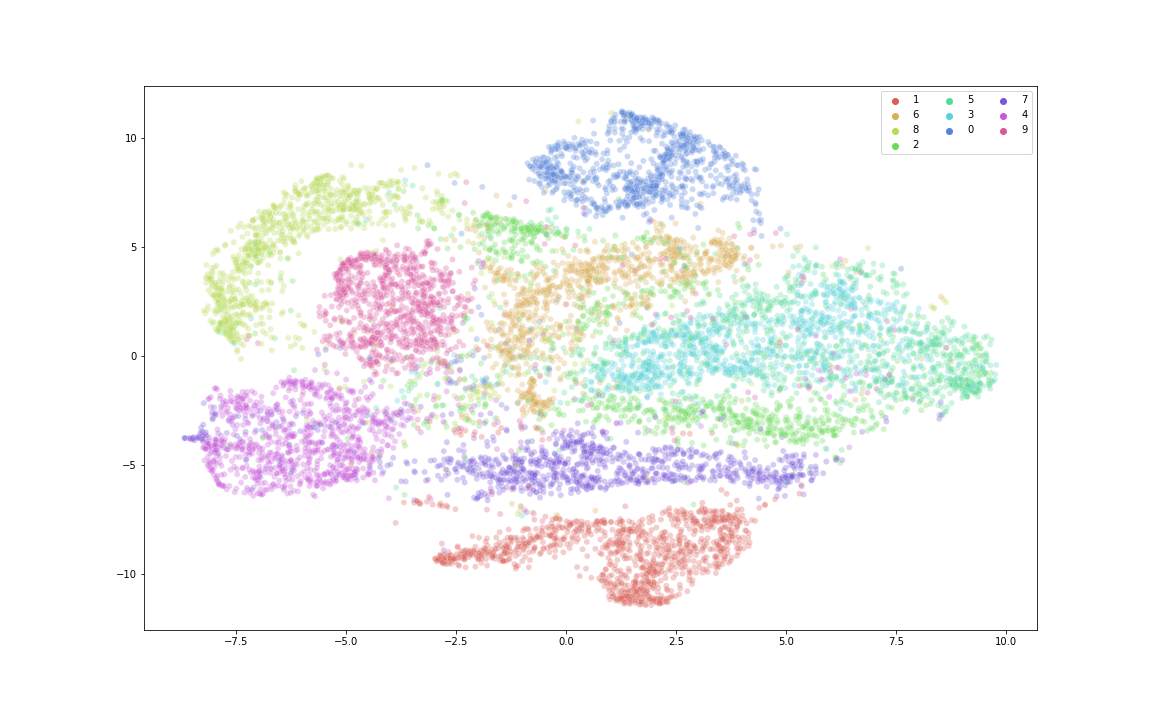
\includegraphics[width=\linewidth]{Final project/img/MNIST_vit-base-patch32-384_train.png}
        \caption{ViT - MNIST}
    \end{subfigure}
    \begin{subfigure}{.48\textwidth}
        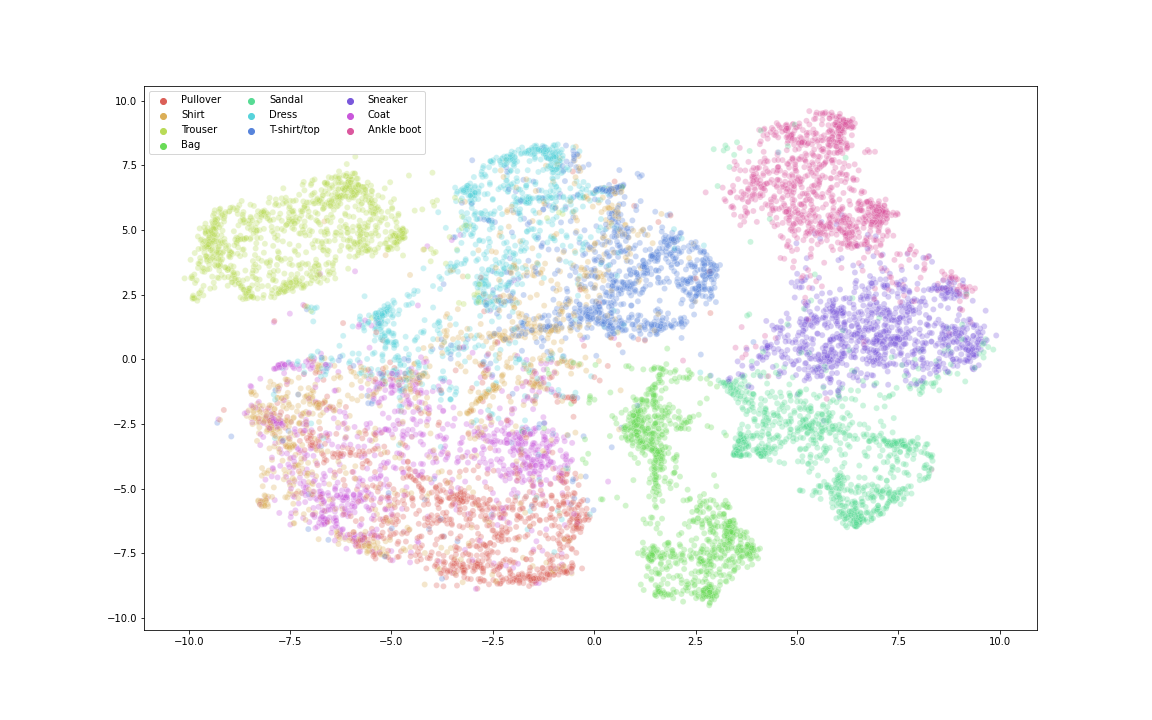
\includegraphics[width=\linewidth]{Final project/img/FMNIST_vit-base-patch32-384_train.png}
        \caption{ViT - FMNIST}
    \end{subfigure}
    \caption{t-SNE Plots for MNIST and Fashion MNIST}
    \label{fig:tsne2}
\end{figure*}

\begin{figure*}[h!]
    \centering
    \begin{subfigure}{.48\textwidth}
        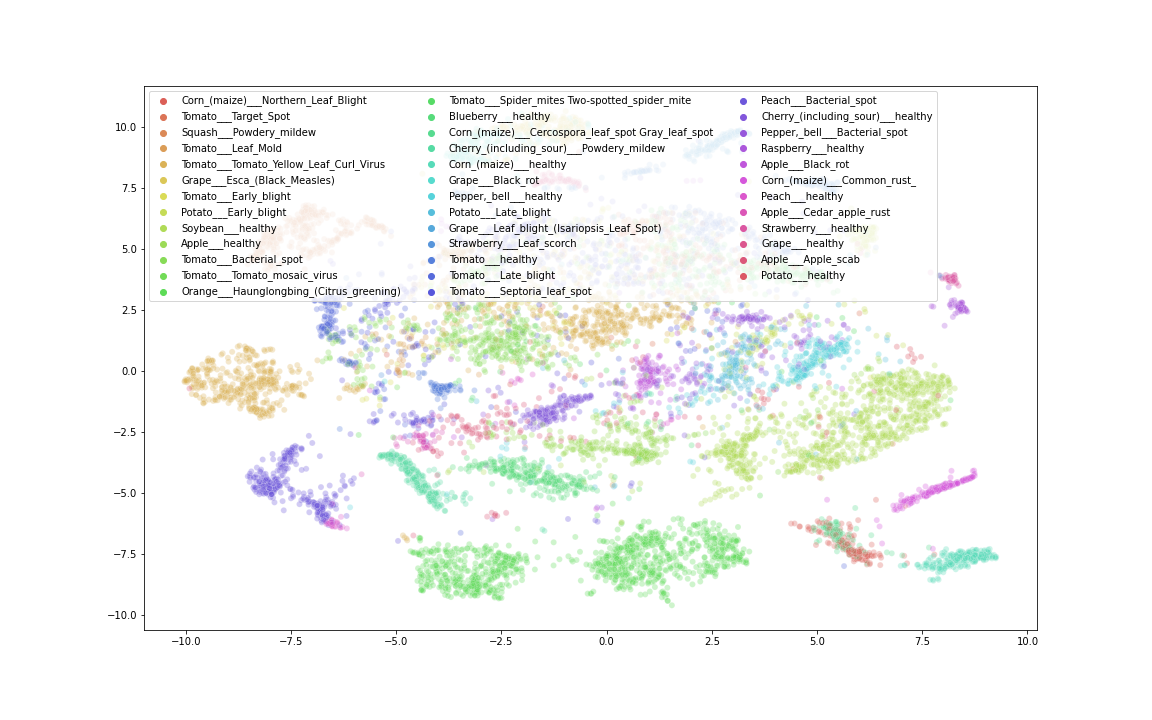
\includegraphics[width=\linewidth]{Final project/img/PlantDisease_RESNET50.png}
        \caption{ResNet50 - PlantDisease}
    \end{subfigure}
    \begin{subfigure}{.48\textwidth}
        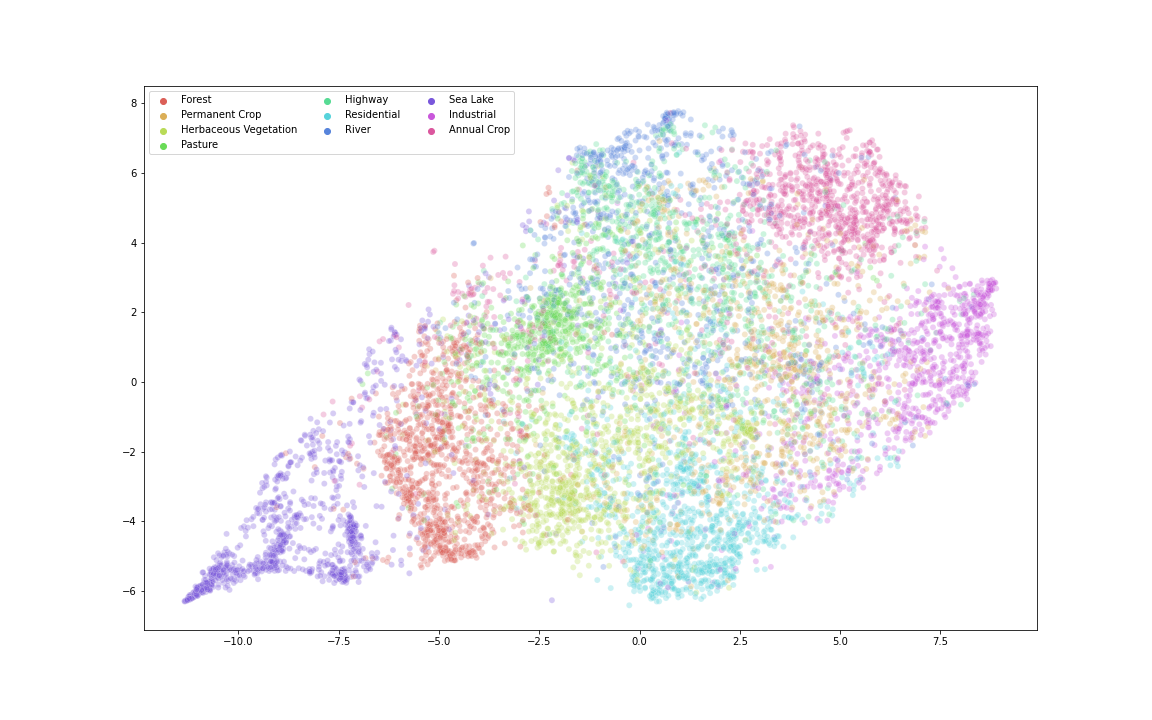
\includegraphics[width=\linewidth]{Final project/img/EuroSAT_RESNET50.png}
        \caption{ResNet50 - EuroSAT}
    \end{subfigure}
    \begin{subfigure}{.48\textwidth}
        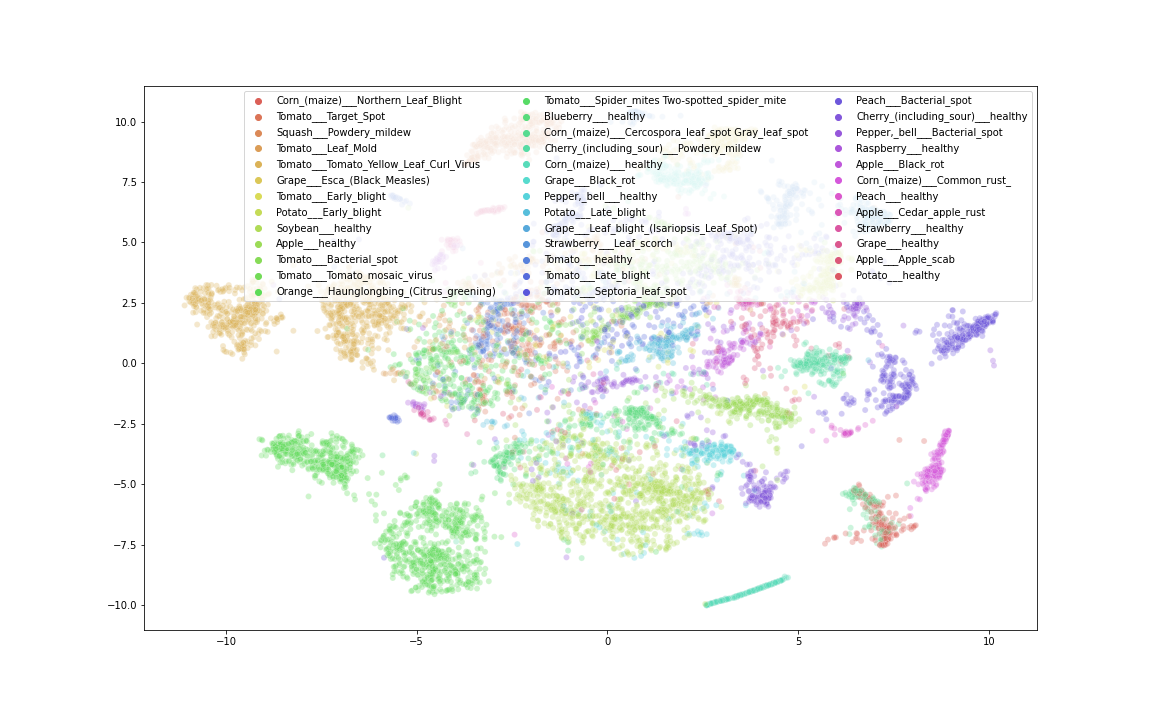
\includegraphics[width=\linewidth]{Final project/img/PlantDisease_clip-vit-base-patch32.png}
        \caption{CLIP - PlantDisease}
    \end{subfigure}
    \begin{subfigure}{.48\textwidth}
        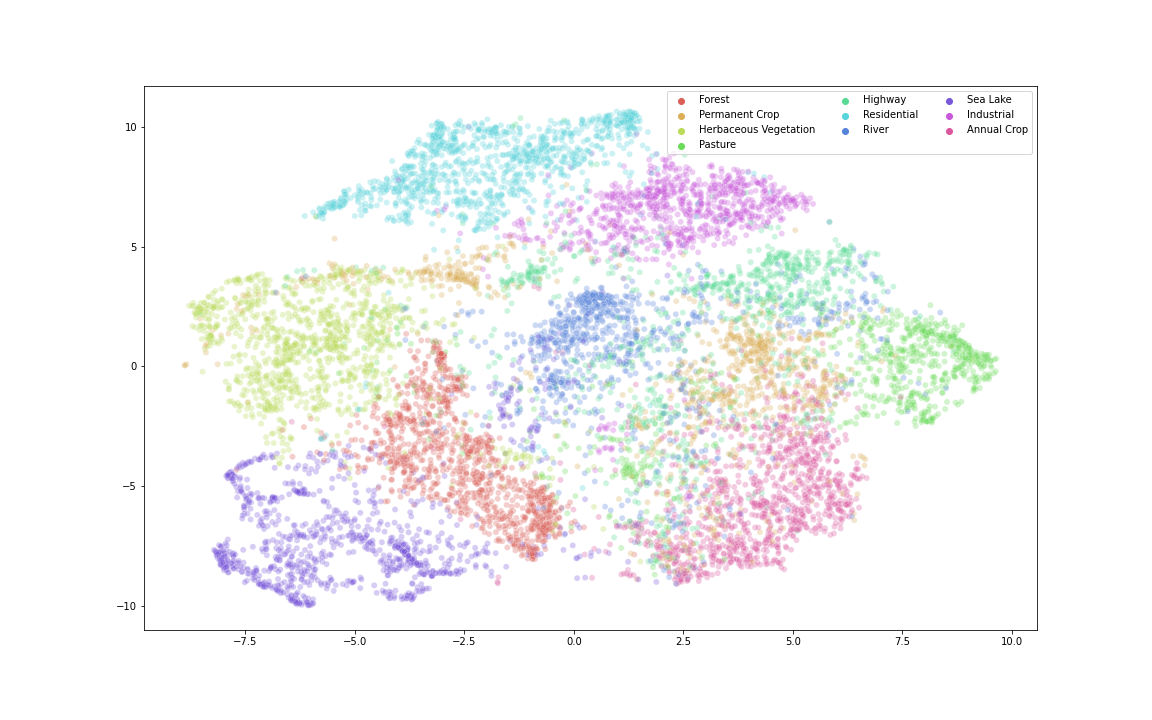
\includegraphics[width=\linewidth]{Final project/img/EuroSAT_clip-vit-base-patch32.png}
        \caption{CLIP - EuroSAT}
    \end{subfigure}
    \begin{subfigure}{.48\textwidth}
        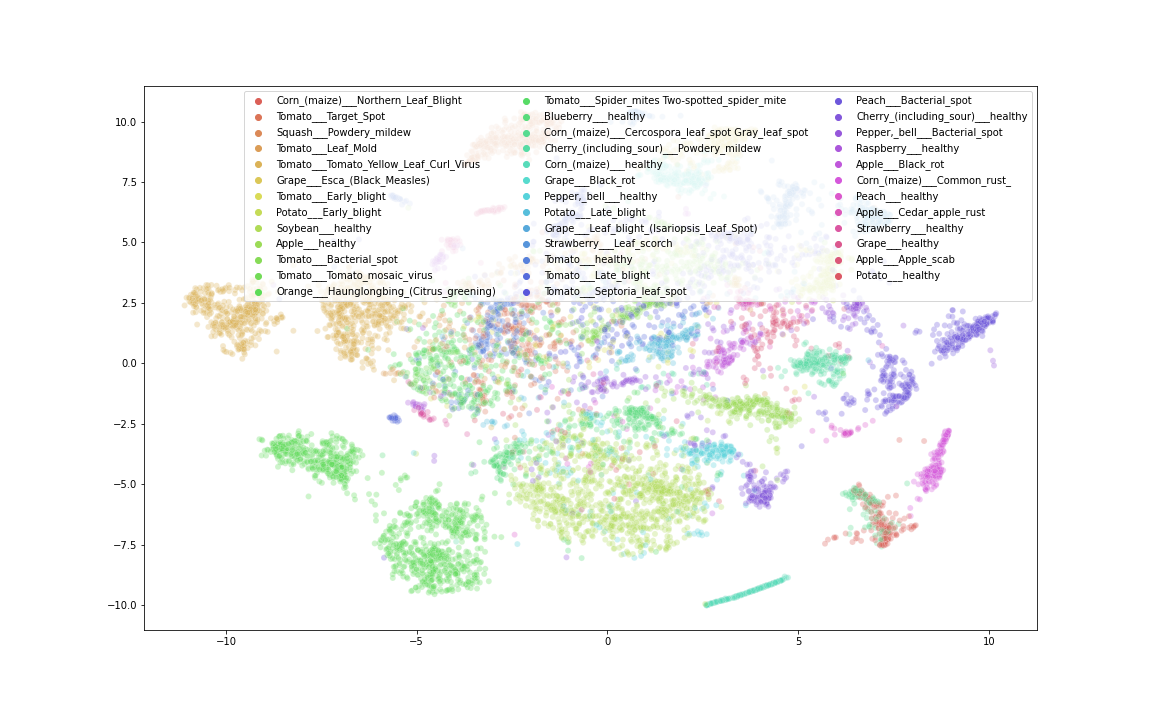
\includegraphics[width=\linewidth]{Final project/img/PlantDisease_clip-vit-base-patch32.png}
        \caption{ViT - PlantDisease}
    \end{subfigure}
    \begin{subfigure}{.48\textwidth}
        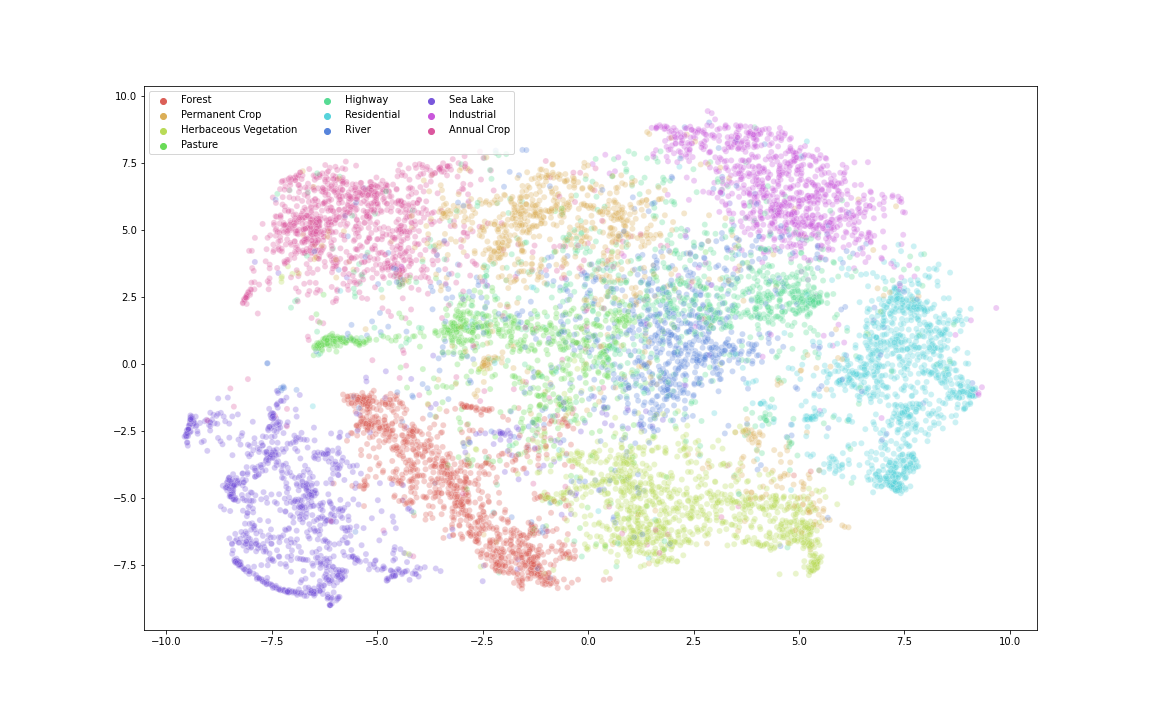
\includegraphics[width=\linewidth]{Final project/img/EuroSAT_vit-base-patch32-384.png}
        \caption{ViT - EuroSAT}
    \end{subfigure}
    \caption{t-SNE Plots for PlantDisease and EuroSAT}
    \label{fig:tsne3}
\end{figure*}

\begin{figure*}[h!]
    \centering
    \begin{subfigure}{.65\textwidth}
        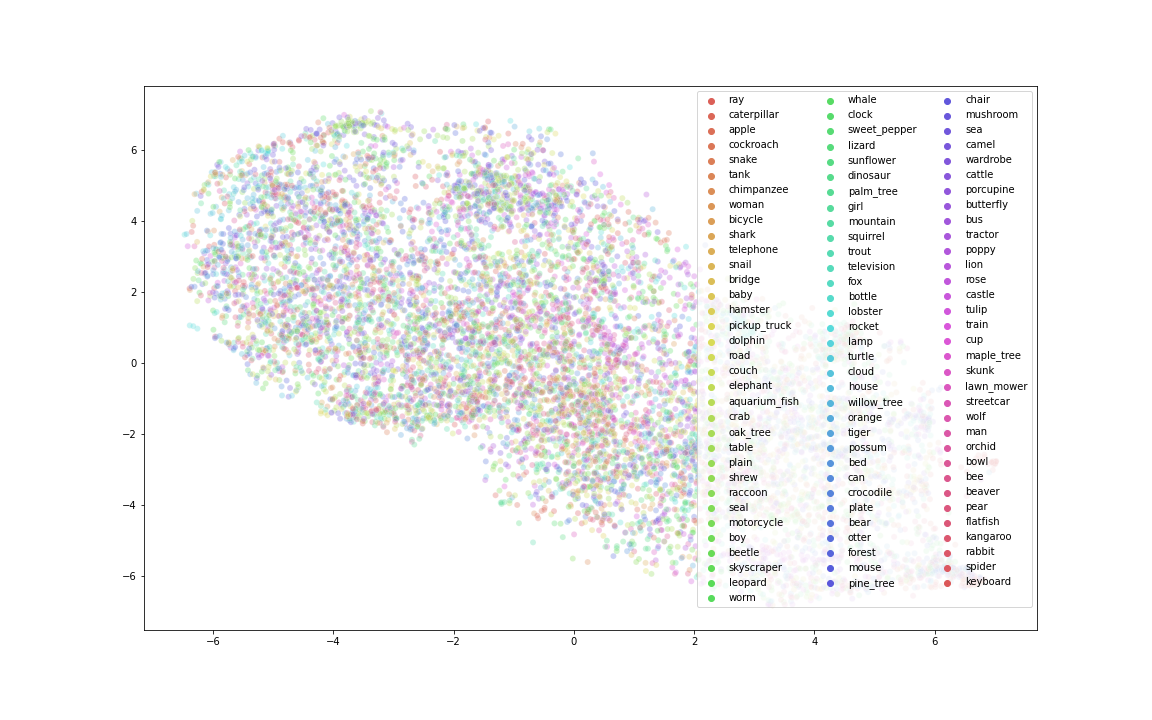
\includegraphics[width=\linewidth]{Final project/img/CIFAR100_RESNET50_train.png}
        \caption{ResNet50 - CIFAR-100}
    \end{subfigure}
    \begin{subfigure}{.65\textwidth}
        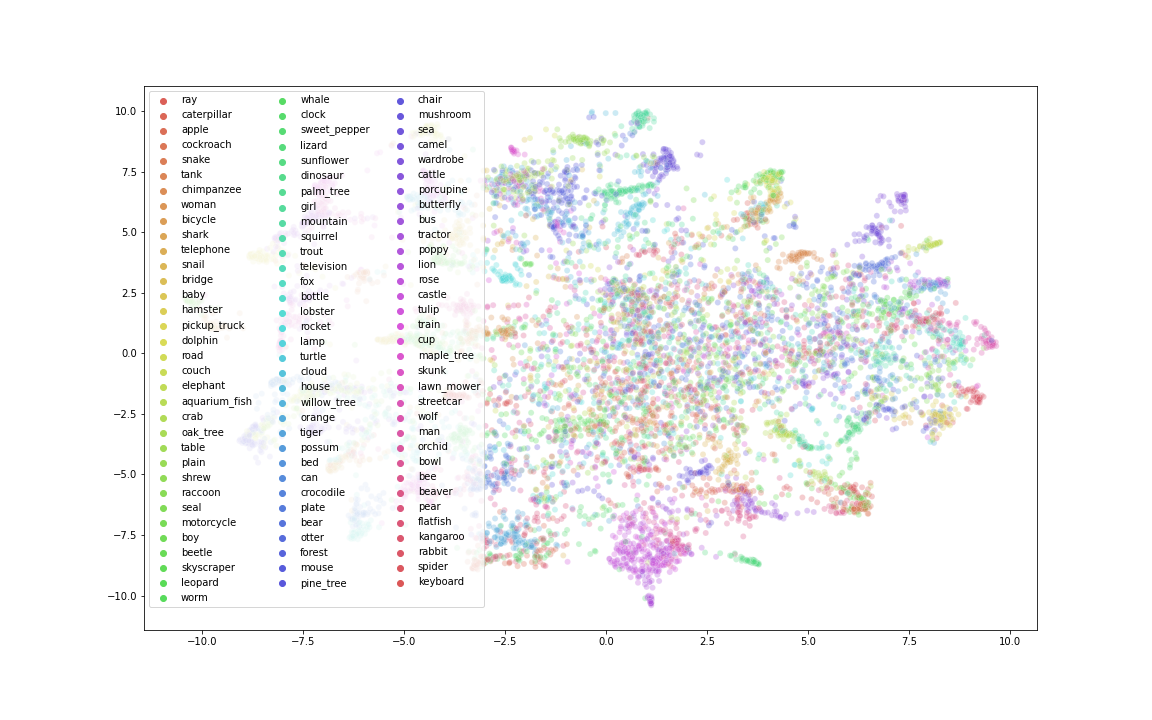
\includegraphics[width=\linewidth]{Final project/img/CIFAR100_clip-vit-base-patch32_train.png}
        \caption{ResNet50 - CIFAR-100}
    \end{subfigure}
    \begin{subfigure}{.65\textwidth}
        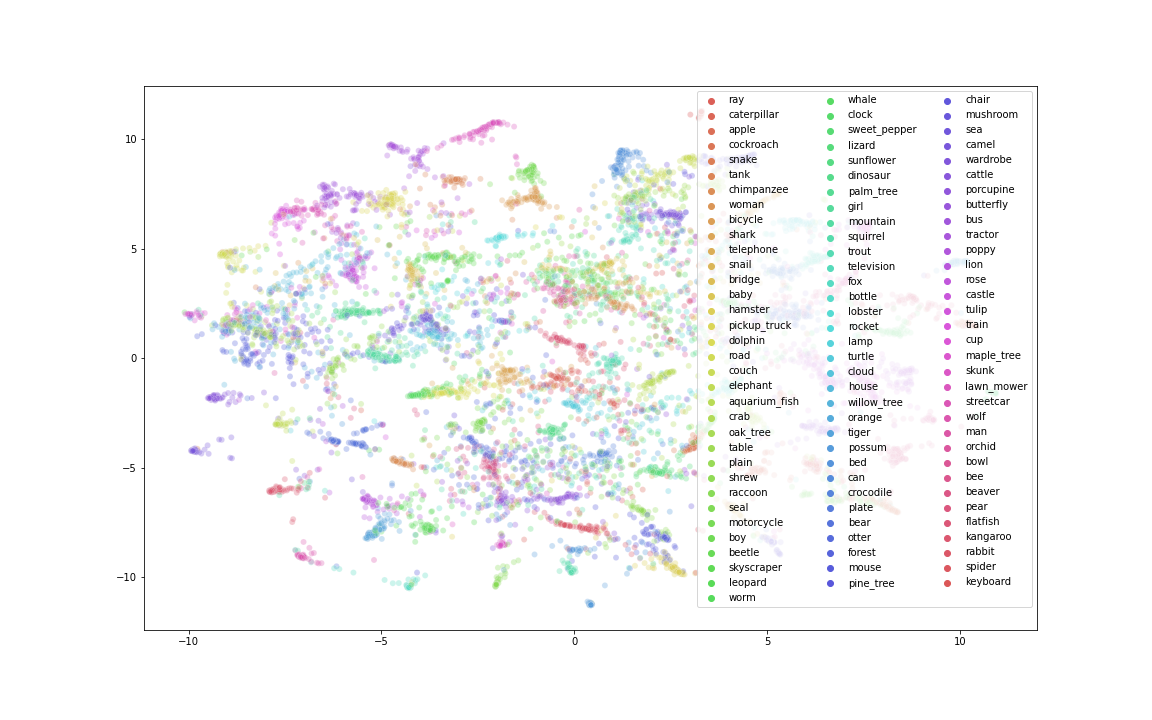
\includegraphics[width=\linewidth]{Final project/img/CIFAR100_vit-base-patch32-384_train.png}
        \caption{CLIP - CIFAR-100}
    \end{subfigure}
    \caption{t-SNE Plots for CIFAR-100}
    \label{fig:tsne4}
\end{figure*}

%%%%%%%%%%%%%%%%%%%%%%%%%%%%%%%%%%%%%%%%%%%%%%%%%%%%%%%%%%%%%%%%%%%%%%%%%%%%%%%
%%%%%%%%%%%%%%%%%%%%%%%%%%%%%%%%%%%%%%%%%%%%%%%%%%%%%%%%%%%%%%%%%%%%%%%%%%%%%%%


\end{document}


% This document was modified from the file originally made available by
% Pat Langley and Andrea Danyluk for ICML-2K. This version was created
% by Iain Murray in 2018, and modified by Alexandre Bouchard in
% 2019 and 2020. Previous contributors include Dan Roy, Lise Getoor and Tobias
% Scheffer, which was slightly modified from the 2010 version by
% Thorsten Joachims & Johannes Fuernkranz, slightly modified from the
% 2009 version by Kiri Wagstaff and Sam Roweis's 2008 version, which is
% slightly modified from Prasad Tadepalli's 2007 version which is a
% lightly changed version of the previous year's version by Andrew
% Moore, which was in turn edited from those of Kristian Kersting and
% Codrina Lauth. Alex Smola contributed to the algorithmic style files.
